\documentclass[../doc.tex]{subfiles}

\begin{document}
    \section{Contrôles du personnage}
        \subsection{Déplacement du joueur}
            Nous avons décider de créer des controleurs avec une vue à la troisième personne.
            Notre jeu sera pour le moment, jouable uniquement au clavier-souris.
            \begin{figure}[hbt!]
                \centering
                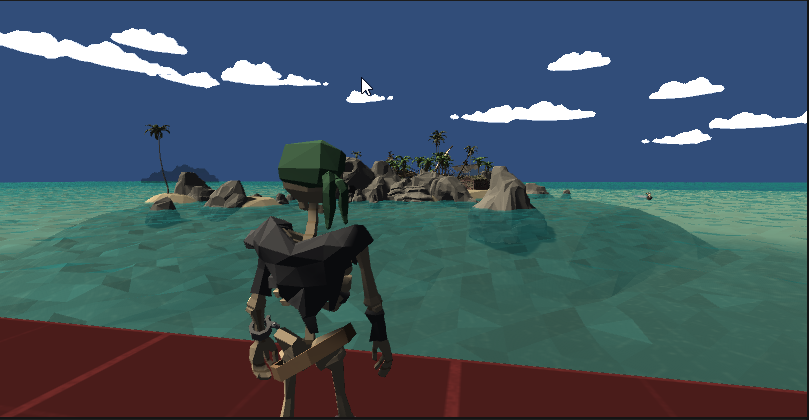
\includegraphics[scale=0.4]{thirdPerson.png}
                \caption{Vue à la troisième personne}
            \end{figure}
            Pour animer les mouvements des joueurs et des NPC, nous avons utilisé la banque d'animations Mixamo que propose Adobe.
            En plus d'avoir des animations détaillées, elles sont entièrement compatible avec le moteur 3D.
            \begin{figure}[hbt!]
                \centering
                \begin{subfigure}[b]{0.3\textwidth}
                    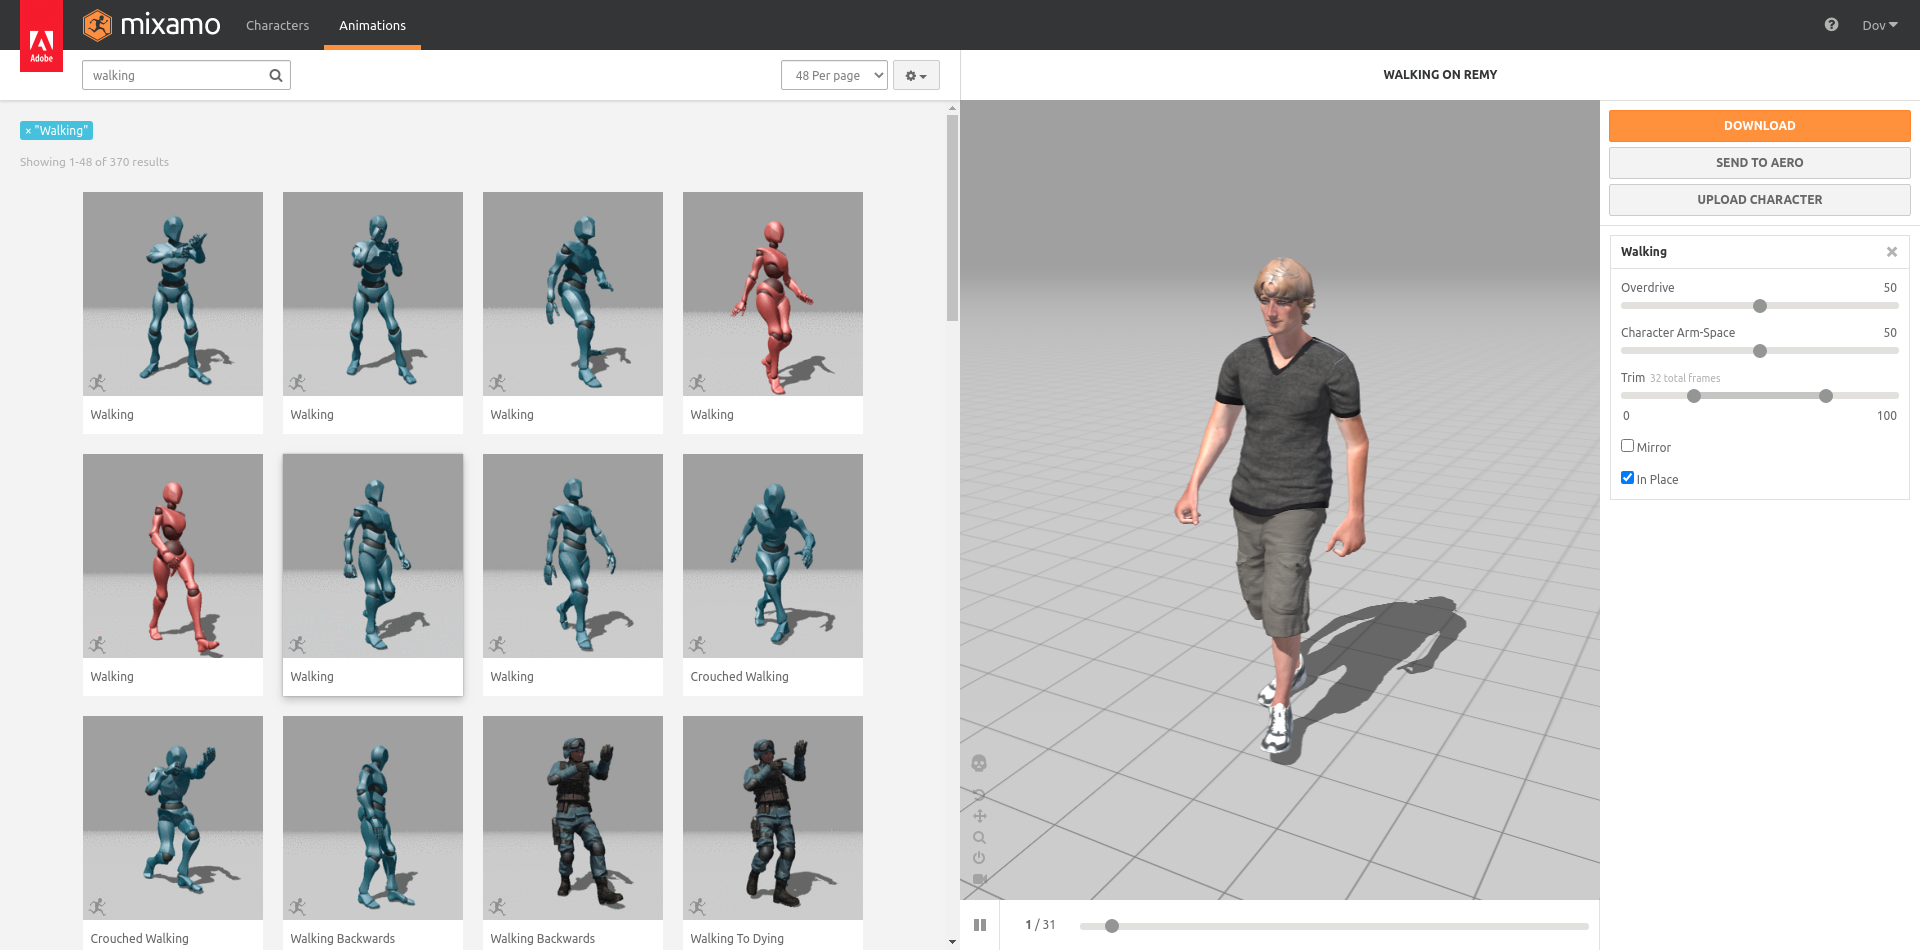
\includegraphics[scale=0.1]{mixamo.png} 
                    \caption{Banque d'animations Mixamo}
                \end{subfigure}
                \hspace{150pt}
                \begin{subfigure}[b]{0.3\textwidth}
                    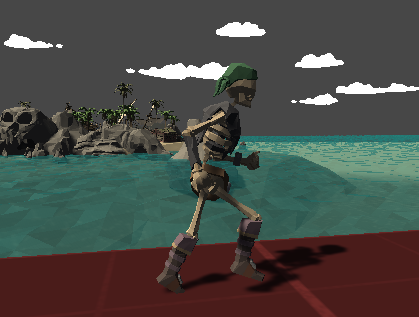
\includegraphics[scale=0.5]{running.png} 
                    \caption{Animation de course sur un personnage}
                \end{subfigure}
                \caption{Animations de Mixamo vers Unity}
            \end{figure}

            Nous avons également choisi d'intégrer des échelles pour permettre aux joueurs de grimper et pour pouvoir rajouter de la verticalité à notre carte\footnote{Voir la partie : Création de la carte}
            \begin{figure}[hbt!]
                \centering
                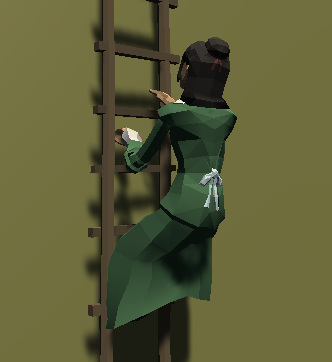
\includegraphics{ladder.png}
                \caption{Joueur grimpant sur l'échelle}
            \end{figure}
        \subsection{Contrôle de la caméra}

            Pour le contrôle de la caméra, nous utiliserons une vue à la troisième personne
            avec possibilité de changer la caméra d'épaule
            Nous avons déjà implémenté une caméra de base, mais qui pose deux problèmes :
            \begin{itemize}
                \item La caméra peut traverser les obstacles si le joueur à le dos collé au mur.
                \item La caméra force la vision du joueur devant lui, ce qui signifie que quand quand le joueur tourne la tête, le personnage aussi, il ne peut donc regarder en arrière. 
            \end{itemize}
            
            Pour régler ce problème, nous prendrons l'outil Cinemachine qui permet en plus de faire des travelings, transitions, possède des caméras adaptées.

\end{document}